\chapter{Problemstellung und Stand der Technik}
\label{ch:problemstellung}

Die thermische Auslegung des Kühlkreislaufs stellt bei der Entwicklung eines Formula Student Fahrzeugs eine der kritischsten Herausforderungen dar. Die aktuelle Problematik lässt sich in zwei Hauptbereiche unterteilen: eine unzureichende empirische Datenbasis sowie eine nachweislich unterdimensionierte Kühlkapazität unter Wettbewerbsbedingungen.

\section{Mangelnde Informationsgrundlage}
\label{sec:informationsgrundlage}

Ein fundamentales Hindernis bei der Dimensionierung des Kühlsystems ist die fehlende Datenbasis zur Bestimmung der thermischen Lasten.

\begin{itemize}
    \item \textbf{Verlustleistungsbestimmung:} Es liegen keine validierten Modelle oder Messreihen vor, um die Verlustleistung der Hauptkomponenten -- Akkumulator, Inverter und Elektromotoren -- über einen gesamten Fahrzyklus zu quantifizieren. Dies ist die grundlegende Ursache aller nachgelagerten Dimensionierungsprobleme.
    \item \textbf{Dimensionierungsrisiko:} Ohne die Kenntnis der tatsächlichen Wärmeströme basiert die Auslegung der Radiatoren und Pumpenleistungen auf Schätzungen. Dies führt entweder zu Mehrgewicht durch Überdimensionierung oder -- wie im vorliegenden Fall -- zu thermischer Überlastung im Betrieb.
    \item \textbf{Lückenhaftes Sensornetz:} Die aktuell erfassten Messgrößen beschränken sich im Wesentlichen auf Komponententemperaturen. Entscheidende Größen wie der Volumenstrom im Kühlkreislauf werden nicht gemessen, wodurch eine vollständige Systemanalyse nicht möglich ist. Dass Felgenbetten durch Infrarotstrahlung der Bremsscheiben schmolzen, ohne dass ein Sensor in diesem Bereich vorhanden war, verdeutlicht diese Lücke exemplarisch.
    \item \textbf{Fehlende thermische Simulation:} Aktuell wird das Kühlsystem gebaut und anschließend im Fahrbetrieb erprobt. Eine vorgelagerte Simulation -- etwa auf Basis eines Lumped-Parameter-Modells -- würde kostspielige Iterationen am realen Fahrzeug reduzieren und eine gezieltere Auslegung ermöglichen.
\end{itemize}

Die folgenden Messdaten illustrieren die Konsequenzen dieser Datenlücken im realen Wettbewerbsbetrieb.

\section{Analyse der thermischen Unterdimensionierung}
\label{sec:thermische_analyse}

Die Auswertung der Telemetriedaten vergangener Testtage und Wettbewerbe verdeutlicht die Defizite des aktuellen Systems. Während Teilsysteme wie der Inverter und der Akkumulator innerhalb der spezifizierten Betriebsgrenzen verbleiben, zeigen die Antriebseinheiten ein kritisches thermisches Verhalten.

\subsection{Vergleich: Testbetrieb vs. Wettbewerbslast}

\paragraph{Testtag (Vorbereitung FSG):}
\begin{figure}[H]
    \centering
    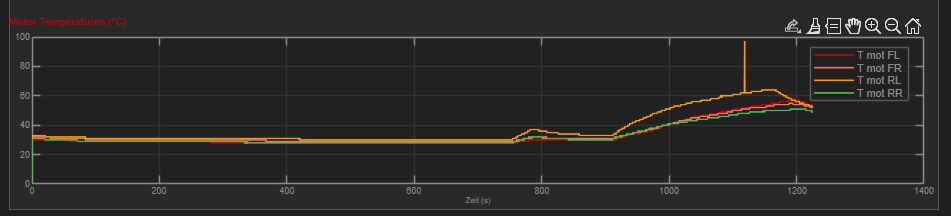
\includegraphics[width=1.0\textwidth]{pics/1.Testtage.jpeg}
    \caption{Temperaturverlauf während der Testphase: Der Motor \textit{Rear Left} (gelbe Kurve) zeigt eine überproportionale Erwärmung gegenüber den übrigen Antriebseinheiten bei moderater Last.}
    \label{fig:log_testtag}
\end{figure}

In dieser Phase zeigten sich erste Auffälligkeiten. Der hintere linke Motor (\textit{Rear Left}) wies eine deutlich höhere Temperaturzunahme auf als die übrigen Motoren. Die Inverter-Temperaturen verharrten auf einem unkritischen Niveau, was auf Potential zur Reduktion der Kühlleistung in diesem Zweig hindeutet. Die Zelltemperaturen des Akkumulators verliefen homogen und innerhalb der Zielparameter.

\paragraph{Endurance FSG:}
\begin{figure}[H]
    \centering
    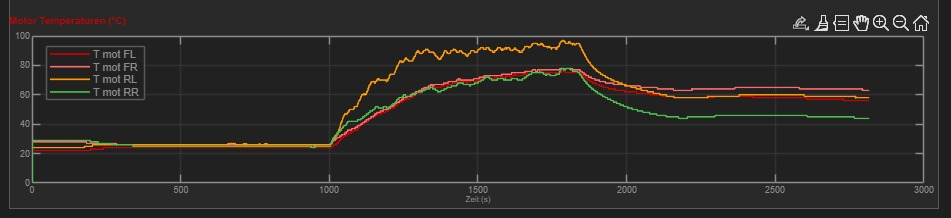
\includegraphics[width=1.0\textwidth]{pics/FSG_Endu_mit_Derating.jpeg}
    \caption{Telemetrie-Log FSG Endurance: Der \textit{Rear Left} Motor erreicht die De-Rating-Schwelle von $90\,^\circ\text{C}$, woraufhin das Managementsystem die Systemleistung automatisch begrenzt.}
    \label{fig:log_fsg_derating}
\end{figure}

Unter Wettbewerbsbedingungen verschärfte sich die Situation deutlich. Während die Frontmotoren und der hintere rechte Motor unterhalb der De-Rating-Grenze von $90\,^\circ\text{C}$ blieben, stagnierte der Motor \textit{Rear Left} bei ca. $100\,^\circ\text{C}$. Das Managementsystem griff daraufhin automatisch ein und drosselte die elektrische Leistung zum Schutz der Hardware, was einen messbaren Performanceverlust zur Folge hatte.

\paragraph{Endurance FS ATA:}
\begin{figure}[H]
    \centering
    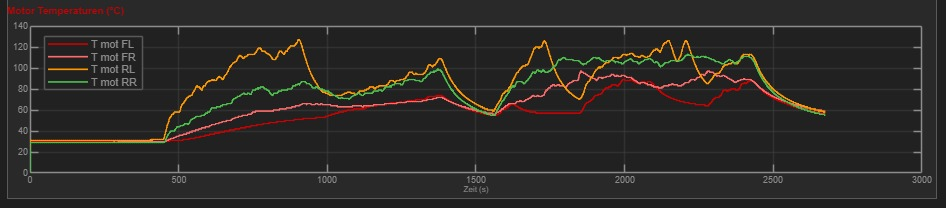
\includegraphics[width=1.0\textwidth]{pics/FSATA_Endu_mit_Abschlatung.jpeg}
    \caption{Thermische Grenzbelastung im FS ATA Endurance: Nach Deaktivierung des De-Ratings kam es bei Temperaturen über $120\,^\circ\text{C}$ zu insgesamt fünf Notabschaltungen (\textit{Engine-Cutoffs}).}
    \label{fig:log_ata_cutoffs}
\end{figure}

Um die Leistungsdrosselung zu umgehen, wurde das De-Rating für den Wettbewerb in Italien deaktiviert. Der Hardwareschutz erfolgte damit ausschließlich durch Notabschaltung. Infolgedessen kam es während des Rennens zu fünf temperaturbedingten Abschaltungen, die den Rennverlauf erheblich beeinträchtigten.

\subsection{Asymmetrisches Thermoverhalten der Antriebseinheiten}
\label{subsec:asymmetrie}

Ein bisher ungeklärter Befund ist das konsistent abweichende Temperaturverhalten des Motors \textit{Rear Left}. Dieser überschreitet in nahezu allen aufgezeichneten Betriebssituationen als erster die kritischen Schwellwerte, während die übrigen drei Motoren deutlich kühler bleiben. Mögliche Ursachen liegen in einer ungleichmäßigen Durchflussverteilung im Kühlkreislauf, in der geometrischen Anordnung der Kühlanbindung oder in einer mechanischen Ursache, die zu erhöhter lokaler Verlustleistung führt. Dieser Befund ist bislang nicht systematisch untersucht worden und stellt einen eigenständigen Analyseschwerpunkt dieser Arbeit dar.

\subsection{Kritische thermische Wechselwirkungen mit der Bremsanlage}
\label{subsec:bremse}

\begin{figure}[htbp]
    \centering
    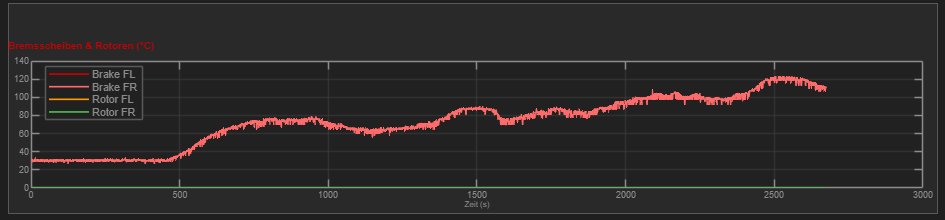
\includegraphics[width=0.9\textwidth]{pics/Brake_Temp_FS_ATA.PNG}
    \caption{Thermische Belastung der Bremsperipherie: Der Anstieg der Rotortemperatur auf über $100\,^\circ\text{C}$ korreliert zeitlich mit den gemeldeten Fading-Effekten und der Infrarot-Abstrahlung auf das Felgenbett.}
    \label{fig:brems_log_ata}
\end{figure}

Zusätzlich zur thermischen Belastung der Antriebskomponenten wurde die Bremsanlage als weiterer kritischer Wärmeeintrag identifiziert:

\begin{itemize}
    \item \textbf{Bremsversagen (Fading):} Temperaturen von über $100\,^\circ\text{C}$ an der Bremsperipherie führten zu einem deutlichen Nachlassen der Bremswirkung und beeinträchtigten die Fahrsicherheit.
    \item \textbf{Strukturelles Versagen durch Strahlungswärme:} In der Saison 2024 führte die Infrarotstrahlung der Bremsscheiben zum Schmelzen der Felgenbetten -- ein Schadensfall, der durch geeignete Messtechnik und thermische Schutzmaßnahmen hätte verhindert werden können.
\end{itemize}

\section{Gewicht-Kühlleistung-Zielkonflikt}
\label{sec:tradeoff}

Die Dimensionierung des Kühlsystems unterliegt einem grundlegenden Zielkonflikt: Größere Radiatoren und leistungsstärkere Pumpen verbessern die Wärmeabfuhr, erhöhen jedoch Gewicht und aerodynamischen Widerstand -- beides kritische Größen im Formula Student Kontext. Ohne ein quantitatives Modell der tatsächlich abzuführenden Wärmemengen kann dieser Trade-off nicht rational bewertet werden. Die bisherige Auslegung basierte auf Erfahrungswerten, was die beschriebenen Probleme begünstigt hat.

\section{Auslegungspunkt und Umgebungsbedingungen}
\label{sec:auslegungspunkt}

Ein weiterer ungeklärter Aspekt betrifft den thermischen Auslegungspunkt des Gesamtsystems. Die Wettbewerbe finden unter unterschiedlichen klimatischen Bedingungen statt: Die FSG in Deutschland und die FS ATA in Italien unterscheiden sich sowohl in Umgebungstemperatur als auch in Luftfeuchtigkeit erheblich. Es ist aktuell nicht definiert, für welche Umgebungsbedingungen das Kühlsystem ausgelegt ist und ob die gewählte Auslegung die ungünstigsten zu erwartenden Bedingungen abdeckt. Dies erschwert eine belastbare Bewertung der Systemreserven.

\section{Historische Analyse der Endurance-Zuverlässigkeit}
\label{sec:historie}

Um die Relevanz einer verbesserten Kühlungsstrategie zu verdeutlichen, fasst Tabelle~\ref{tab:endurance_historie} die Ergebnisse der vergangenen Endurance-Läufe sowie die jeweiligen Hauptursachen für Ausfälle oder Leistungseinschränkungen zusammen.

\begin{table}[htbp]
    \centering
    \caption{Analyse der Endurance-Ergebnisse von 2021 bis 2025}
    \label{tab:endurance_historie}
    \small
    \renewcommand{\arraystretch}{1.25}
    \begin{tabularx}{\textwidth}{|l|l|l|X|}
        \hline
        \textbf{Jahr} & \textbf{Event} & \textbf{Status} & \textbf{Primäre Ausfallursache / Problem} \\
        \hline\hline
        2021 & FSG    & DNF    & Elektrische Defekte (LV-Platine) \\
        2022 & FSG    & DNS    & Defekt im Akkumulator-Container \\
        2023 & FSG    & DNS    & Mechanisches Versagen (Radaufhängung) \\
        2023 & FSAA   & DNF    & Mechanisches Versagen (Radaufhängung) \\
        \hline
        2024 & FSCZ   & DNF    & \textbf{Thermische Überlastung der Bremse} \\
        2024 & FSG    & DNF    & \textbf{Schmelzende Felgenbetten durch Strahlungshitze} \\
        2024 & FS ATA & Erfolg & Erster erfolgreicher AWD-Endurance \\
        \hline
        2025 & FS CZ  & DNS    & Mechanisches Versagen (Radaufhängung) \\
        2025 & FS G   & DNF    & \textbf{Dichtungsschaden infolge von Überhitzung} \\
        2025 & FS ATA & Erfolg & Zielankunft mit \textbf{5 Engine-Cutoffs} und massiver Leistungsbegrenzung \\
        \hline
    \end{tabularx}
\end{table}

\noindent\small{DNF = Did Not Finish, DNS = Did Not Start}
\vspace{1em}

\subsection{Identifikation des thermischen Bottlenecks}
\label{subsec:bottleneck}

Die Auswertung der vergangenen fünf Jahre zeigt eine deutliche Verschiebung der technischen Herausforderungen. Während in der frühen Phase von 2021 bis 2023 primär grundlegende elektrische und mechanische Zuverlässigkeit im Vordergrund stand, hat sich seit der Einführung des Allradantriebs die thermische Standfestigkeit als kritischer Limitierungsfaktor etabliert.

Besonders die Saisons 2024 und 2025 verdeutlichen, dass das Fahrzeug mechanisch und elektrisch konkurrenzfähig ist, jedoch durch unzureichende Wärmeabfuhr am Erreichen der Ziellinie gehindert wird. Das Schmelzen von Felgenbetten (FSG 2024) sowie thermisch bedingte Dichtungsschäden (FSG 2025) sind klare Indikatoren dafür, dass das thermische System die Grenzen der Betriebssicherheit erreicht hat. Die vorliegende Arbeit setzt genau an diesem Punkt an und zielt darauf ab, die beschriebenen Defizite systematisch zu erfassen und eine fundierte Grundlage für die Auslegung eines verbesserten Kühlsystems zu schaffen.
